\documentclass{beamer}
\usepackage[utf8]{inputenc}

\usepackage{xeCJK}
\usepackage{graphicx} %插入图片的宏包
\usepackage{float} %设置图片浮动位置的宏包
\usepackage{subfigure} %插入多图时用子图显示的宏包

\usetheme{Madrid}
\usecolortheme{default}

\title{2022年秋季招新线上培训}
\subtitle{如何使用ssh连接到集群并开发}
\author{七边形超算队}
\institute{华中科技大学}
\date{2022年11月20日}
\logo{
\includegraphics[height=1cm]{heptagon.jpg}}
\begin{document}

\AtBeginSection[]
{
  \begin{frame}
    \frametitle{目录}
    \tableofcontents[currentsection]
  \end{frame}
}

%\begin{document}

%The next statement creates the title page.
\frame{\titlepage}

%---------------------------------------------------------
%This block of code is for the table of contents after
%the title page
\begin{frame}
\frametitle{目录}
\tableofcontents
\end{frame}
%---------------------------------------------------------


\section{简要介绍}

%---------------------------------------------------------
%Changing visivility of the text
\begin{frame}
\frametitle{What}

\begin{itemize}
    \item<1-> 前提条件:选手已经在自己的电脑上对代码进行了一定程度的优化。
    \item<2-> 什么是ssh 
    
简单说,SSH是一种网络协议,我们用于计算机之间的加密登录。
当在远端有一台机器时,我们可以使用ssh登录到远端的机器,并像在自己的电脑上一样编写代码,运行程序。
    
\end{itemize}

\end{frame}

\begin{frame}
\frametitle{Why}
\begin{itemize}
    \item<1-> 为什么要使用集群
    \item<2-> 集群的配置条件比一般的个人计算机更为优越,尤其是在CPU核数上,我们可以使代码有更高的并行程度。直观来说,就是可以同时使用更多的线程。同时集群会提供统一的环境,便于我们的对选手代码的复核。
\end{itemize}
\end{frame}

\begin{frame}
\frametitle{How}
\begin{itemize}
    \item<1-> 我们会提供什么
    \item<2-> 我们会在集群上为你开设一个账户,你可以使用这个账户远程登录集群
\end{itemize}
\end{frame}

\section{连接集群}

%---------------------------------------------------------
%Highlighting text
\begin{frame}
\frametitle{命令行环境}

\begin{itemize}
    \item<1-> 可以使用命令行终端测试登录
    \item<2-> 输入如下命令:ssh user@host -p 端口号
    
    其中,user使我们为你提供的账户名,host是我们会同时告知你的主机ip地址和端口。之后输入提供的密码即可。
     \item<3-> 提醒:请使用校园网
\end{itemize}

\end{frame}

\begin{frame}
\frametitle{VScode}

\begin{itemize}
    \item<1-> 在vs code中安装Remote Development插件
    \item<2-> 将登录信息写入到config文件
    
    windows下一般为:C:\textbackslash Users\textbackslash 用户名\textbackslash .ssh\textbackslash config
    
    linux和mac下一般为:\textasciitilde/.ssh/config
    
    \item<3-> 通常格式为:
    \begin{figure}[H] %H为当前位置,!htb为忽略美学标准,htbp为浮动图形
    	\centering %图片居中
    	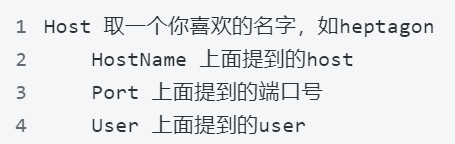
\includegraphics[width=0.7\textwidth]{p1.png} %插入图片,[]中设置图片大小,{}中是图片文件名
    	%\caption{} %最终文档中希望显示的图片标题
    	\label{p1} %用于文内引用的标签
    \end{figure}

\end{itemize}

\end{frame}

\begin{frame}
\frametitle{配置ssh密匙}

\begin{itemize}
    \item<1-> 使用 ssh-keygen 在命令行终端生成ssh密匙
    
    推荐使用默认的保存地址,一般为C:\textbackslash Users\textbackslash 用户名\textbackslash.ssh\textbackslash id\_rsa
    
    在生成过程中的passphrase推荐直接回车,也即不设置密码。
    
    公匙为\textasciitilde\textbackslash.ssh\textbackslash id\_rsa.pub
    
    私匙为\textasciitilde\textbackslash.ssh\textbackslash id\_rsa
    
    \item<2-> 放置
    
    .pub文件放到远端:
    \textasciitilde\textbackslash.ssh\textbackslash authorized\_keys
    \item<3-> 在github上添加公匙
\end{itemize}

\end{frame}


\section{linux等的使用(以ubuntu为例)}

\begin{frame}
\frametitle{常用命令}

\begin{itemize}
    \item<1-> 各类基本命令
    
    touch mkdir rm ls ll ctrl+c ctrl+d
    \item<2-> git的使用
    
    clone
    add
    commit 
    push 
    
    \item<3-> 构建与运行
    
    cmake和make
    ./app args
    添加lib
    \begin{figure}[H] %H为当前位置,!htb为忽略美学标准,htbp为浮动图形
    	\centering %图片居中
    	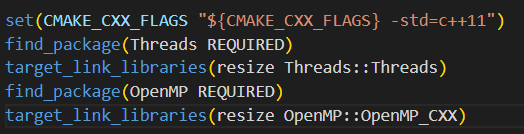
\includegraphics[width=0.7\textwidth]{p2.png} %插入图片,[]中设置图片大小,{}中是图片文件名
    	%\caption{} %最终文档中希望显示的图片标题
    	\label{p2} %用于文内引用的标签
    \end{figure}
    
    
\end{itemize}
\end{frame}


\section{上手}

\begin{frame}{实操}
    
\item 常见问题

\item

\item 常见方法

\item

\item ... 

\end{frame}

\end{document}